% =====================================================================
% appendices/appendix_b_additional_results.tex
% Appendix B — Additional Results
% Project: Vision-Based Running Technique Classification from In-the-Wild
%          Internet Videos using Markerless Pose Estimation and Deep Learning
%
% Required preamble packages in main.tex:
%   \usepackage{booktabs}
%   \usepackage{array}
%   \usepackage{tabularx}
%   \usepackage{graphicx}
%
% This appendix collects supplementary figures and the development version
% history. It does not introduce new controlled benchmark numbers. All figure
% inclusions are guarded by \IfFileExists so that compilation does not fail if
% a supplementary image has not been copied into the LaTeX figures directory.
% =====================================================================

\chapter{Additional Results}
\label{app:additional-results}

This appendix collects supplementary material referenced from
Chapters~\ref{ch:results}--\ref{ch:discussion}: additional confusion matrices,
cycle-detection signal examples, training curves, failed-case summaries, and
the autocorrelation version history. No new controlled benchmark results are
introduced here; the controlled results remain those reported in
Chapter~\ref{ch:results}.

% ---------------------------------------------------------------------
\section{Additional Confusion Matrices}
\label{app:confusion}

\IfFileExists{figures/handmade_confusion_matrix.png}{
\begin{figure}[htbp]
\centering
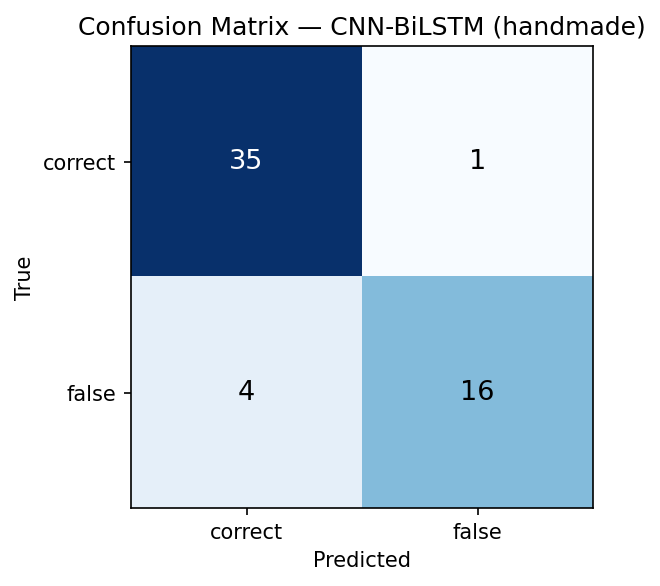
\includegraphics[width=0.60\textwidth]{figures/handmade_confusion_matrix.png}
\caption{Confusion matrix of the best handmade upper-bound model on the test set.}
\label{fig:cm-handmade}
\end{figure}
}{
\noindent\textit{Supplementary figure not available in the LaTeX tree:
\texttt{figures/handmade\_confusion\_matrix.png}.}
}

\IfFileExists{figures/autocorr_confusion_matrix.png}{
\begin{figure}[htbp]
\centering
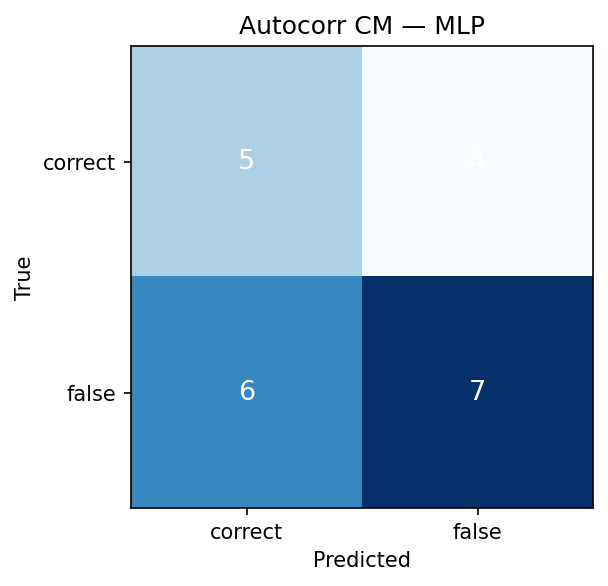
\includegraphics[width=0.60\textwidth]{figures/autocorr_confusion_matrix.png}
\caption{Confusion matrix of the autocorr landmark baseline on the test set.}
\label{fig:cm-autocorr}
\end{figure}
}{
\noindent\textit{Supplementary figure not available in the LaTeX tree:
\texttt{figures/autocorr\_confusion\_matrix.png}.}
}

\IfFileExists{figures/image_confusion_matrix.png}{
\begin{figure}[htbp]
\centering
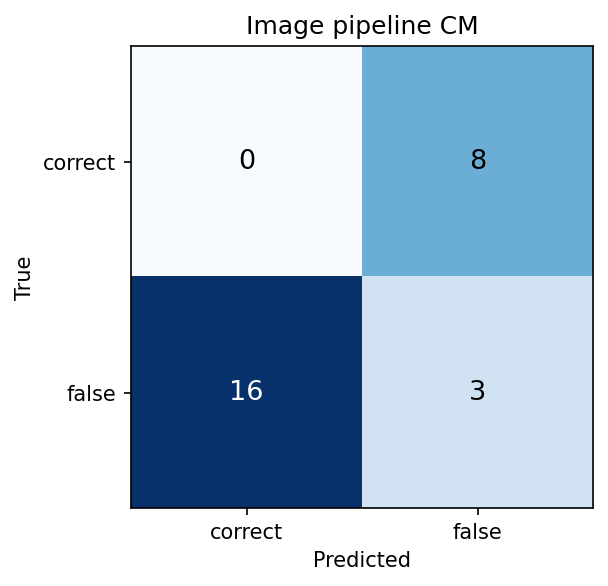
\includegraphics[width=0.60\textwidth]{figures/image_confusion_matrix.png}
\caption{Confusion matrix of the autocorr image-based pipeline on the test set.}
\label{fig:cm-image}
\end{figure}
}{
\noindent\textit{Supplementary figure not available in the LaTeX tree:
\texttt{figures/image\_confusion\_matrix.png}.}
}

% ---------------------------------------------------------------------
\section{Additional Signal Examples}
\label{app:signal-examples}

\IfFileExists{figures/contact_diff_signal_example.png}{
\begin{figure}[htbp]
\centering
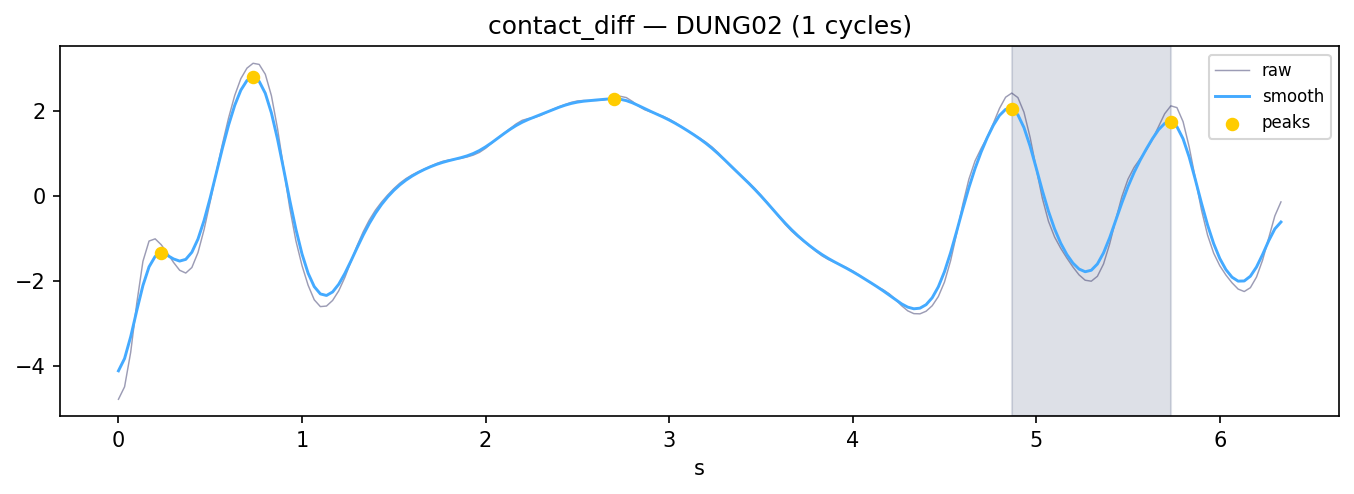
\includegraphics[width=0.80\textwidth]{figures/contact_diff_signal_example.png}
\caption{Example \texttt{contact\_diff} motion signal used for autocorrelation-based cycle detection.}
\label{fig:signal-contactdiff}
\end{figure}
}{
\noindent\textit{Supplementary figure not available in the LaTeX tree:
\texttt{figures/contact\_diff\_signal\_example.png}.}
}

\IfFileExists{figures/detected_cycle_example.png}{
\begin{figure}[htbp]
\centering
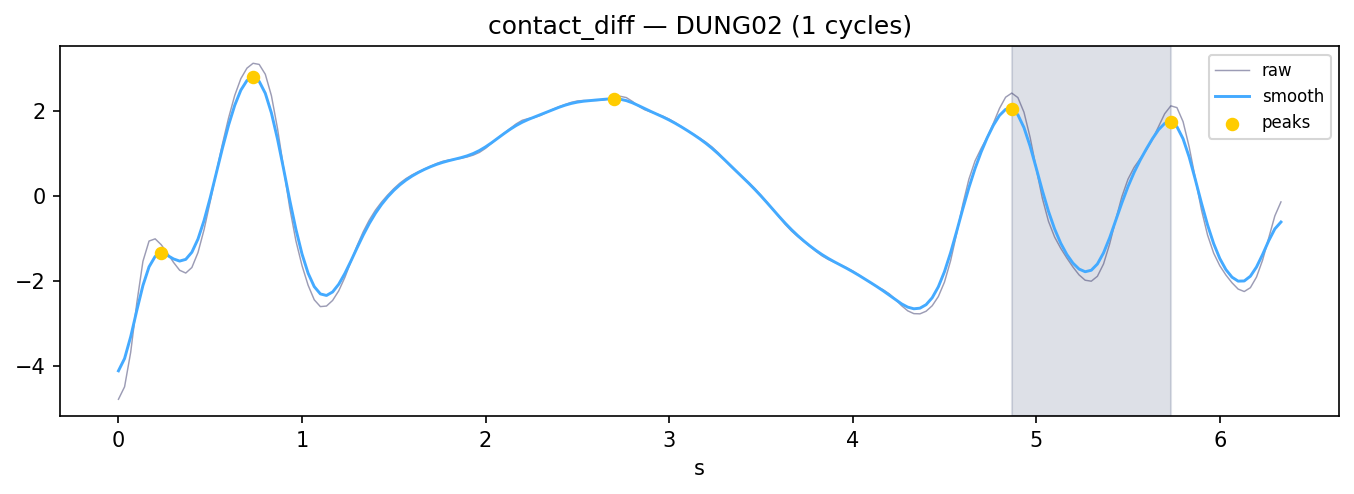
\includegraphics[width=0.80\textwidth]{figures/detected_cycle_example.png}
\caption{Example of an automatically detected foot-strike-to-foot-strike running cycle.}
\label{fig:detected-cycle}
\end{figure}
}{
\noindent\textit{Supplementary figure not available in the LaTeX tree:
\texttt{figures/detected\_cycle\_example.png}.}
}

\IfFileExists{figures/8phase_autocorr_sample.png}{
\begin{figure}[htbp]
\centering
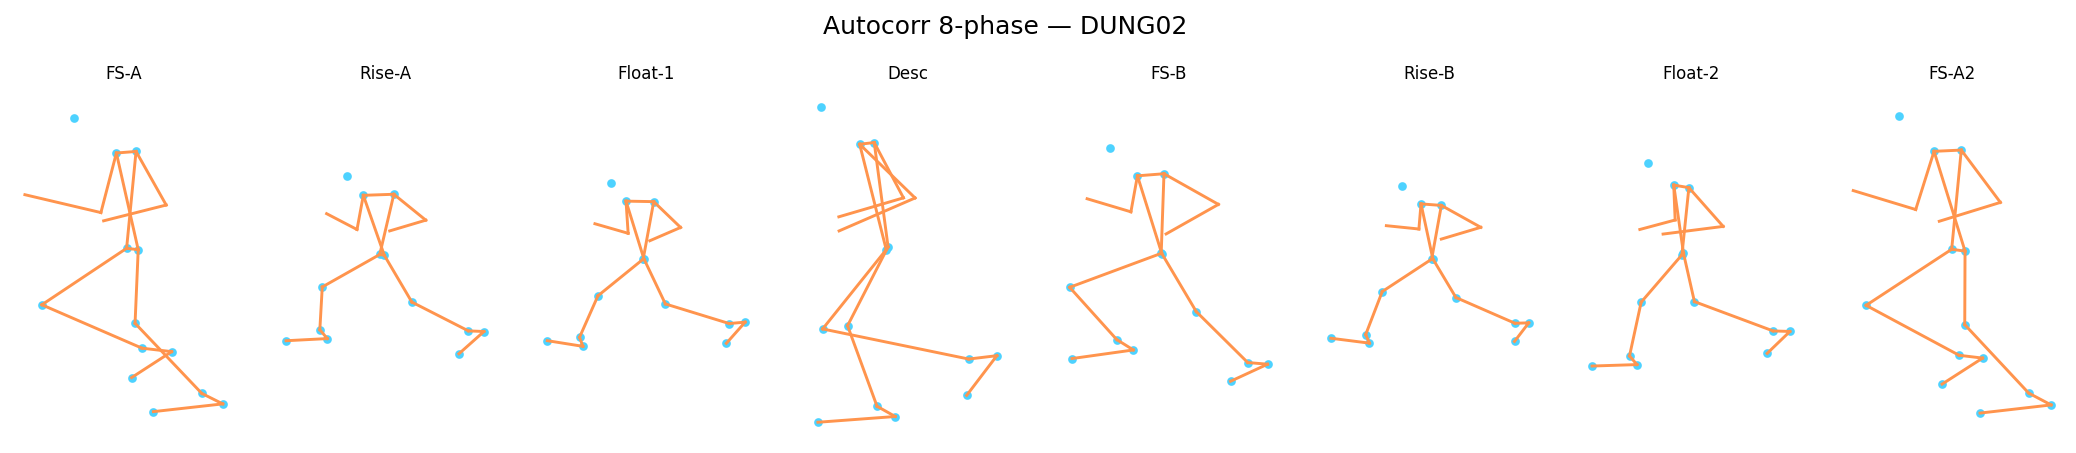
\includegraphics[width=0.80\textwidth]{figures/8phase_autocorr_sample.png}
\caption{Example eight-phase sampling of an automatically detected cycle.}
\label{fig:8phase-autocorr-sample}
\end{figure}
}{
\noindent\textit{Supplementary figure not available in the LaTeX tree:
\texttt{figures/8phase\_autocorr\_sample.png}.}
}

\IfFileExists{figures/period_distribution.png}{
\begin{figure}[htbp]
\centering
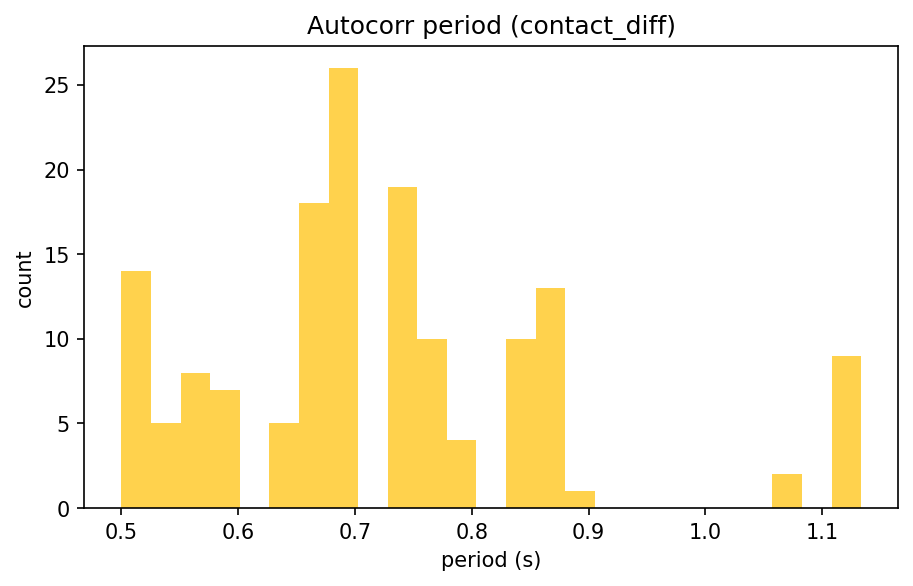
\includegraphics[width=0.70\textwidth]{figures/period_distribution.png}
\caption{Distribution of estimated cycle periods across detected videos.}
\label{fig:period-dist}
\end{figure}
}{
\noindent\textit{Supplementary figure not available in the LaTeX tree:
\texttt{figures/period\_distribution.png}.}
}

% ---------------------------------------------------------------------
\section{Training Curves}
\label{app:training-curves}

\IfFileExists{figures/handmade_training_curve.png}{
\begin{figure}[htbp]
\centering
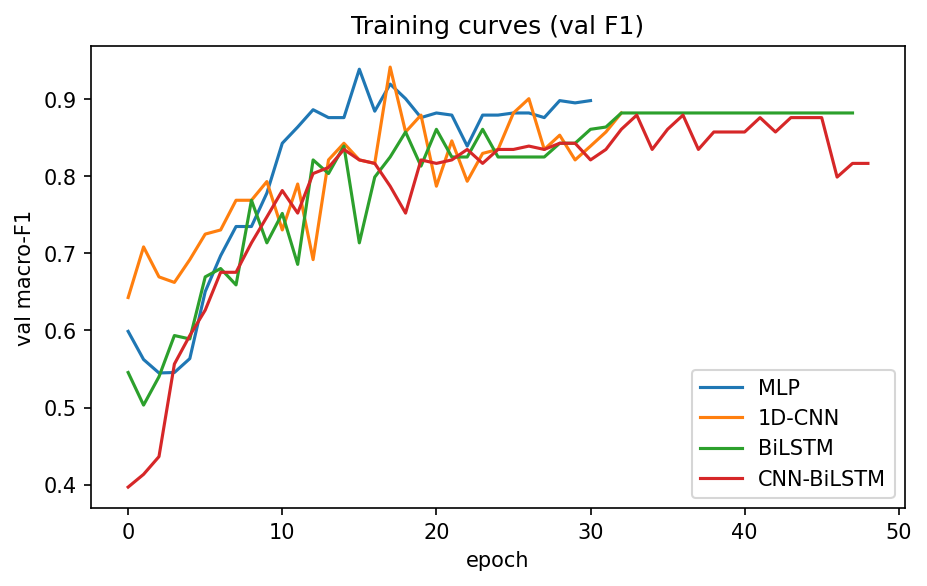
\includegraphics[width=0.80\textwidth]{figures/handmade_training_curve.png}
\caption{Training and validation curves for the handmade upper-bound models.}
\label{fig:curve-handmade}
\end{figure}
}{
\noindent\textit{Supplementary figure not available in the LaTeX tree:
\texttt{figures/handmade\_training\_curve.png}.}
}

\IfFileExists{figures/image_training_curve.png}{
\begin{figure}[htbp]
\centering
\includegraphics[width=0.80\textwidth]{figures/image_training_curve.png}
\caption{Training and validation curves for the autocorr image-based pipeline.}
\label{fig:curve-image}
\end{figure}
}{
\noindent\textit{Supplementary figure not available in the LaTeX tree:
\texttt{figures/image\_training\_curve.png}.}
}

% ---------------------------------------------------------------------
\section{Failed Case Examples}
\label{app:failed-cases}

\IfFileExists{figures/reject_reason_chart.png}{
\begin{figure}[htbp]
\centering
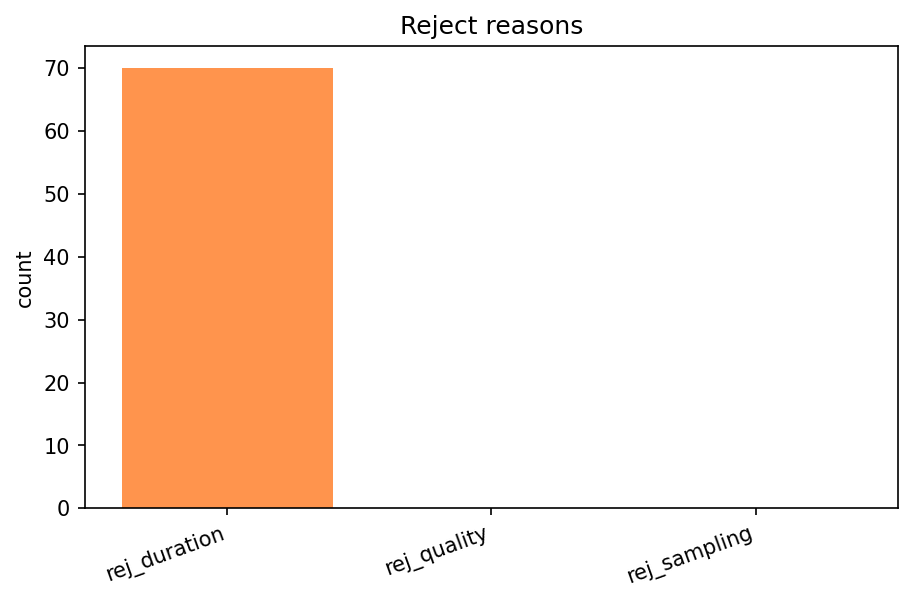
\includegraphics[width=0.70\textwidth]{figures/reject_reason_chart.png}
\caption{Breakdown of cycle-level rejection reasons in the autocorr pipeline.}
\label{fig:reject-reasons}
\end{figure}
}{
\noindent\textit{Supplementary figure not available in the LaTeX tree:
\texttt{figures/reject\_reason\_chart.png}.}
}

The per-video failure records are available in \path{outputs/autocorr/autocorr_failed_videos.csv} and the image-pipeline counterpart \path{outputs/autocorr_image/failed_videos.csv}, when those files are exported by the corresponding notebooks.


% ---------------------------------------------------------------------
\section{Fair Gap Robustness and Permutation Test}
\label{app:fair-gap}

Table~\ref{tab:app-fair-gap} records the supplementary robustness check used in
Section~\ref{sec:fair-gap}. It repeats the handmade--autocorr comparison with
the same MLP classifier, a fixed threshold of $0.5$, and 5-fold video-level
cross-validation. The values support the fixed-split conclusion that automatic
cycle detection is the main bottleneck.

\begin{table}[htbp]
\centering
\caption{Fair-gap robustness check and autocorr MLP permutation test. Source: \texttt{outputs/autocorr/fair\_gap\_and\_mlp\_perm.json}.}
\label{tab:app-fair-gap}
\renewcommand{\arraystretch}{1.18}
\scriptsize
\begin{tabularx}{\textwidth}{X r}
\toprule
\textbf{Quantity} & \textbf{Value} \\
\midrule
Handmade cycles / videos & 370 / 369 \\
Autocorr cycles / videos & 151 / 55 \\
Handmade 5-fold CV macro-F1 & $0.8597 \pm 0.0160$ \\
Handmade OOF macro-F1, 95\% CI & 0.8599 [0.8219, 0.8969] \\
Autocorr 5-fold CV macro-F1 & $0.6146 \pm 0.0809$ \\
Autocorr OOF macro-F1, 95\% CI & 0.6553 [0.5797, 0.7281] \\
Fair gap (handmade $-$ autocorr) & 0.2451 \\
Observed autocorr MLP CV macro-F1 in permutation test & 0.5206 \\
Permutation null mean $\pm$ std. & $0.4680 \pm 0.0740$ \\
Number of permutations & 100 \\
Permutation $p$-value & 0.2475 \\
\bottomrule
\end{tabularx}
\end{table}

The permutation result is interpreted conservatively. It does not prove that the
autocorr cycles contain no signal; it indicates that the signal is not robustly
separable under the tested simple MLP configuration and current sample size.


% ---------------------------------------------------------------------
\section{Autocorr Version History}
\label{app:version-history}

This section reproduces the autocorrelation version history for completeness.
\textbf{These are historical development results, not controlled benchmarks.}
The reported validation accuracies were recorded in development notebooks under
varying protocols and are \emph{not} directly comparable to the controlled
test metrics of Chapter~\ref{ch:results}. In particular,
\texttt{autocorr\_fixed(val\_acc 76.5)} is a historical image-based milestone
that motivated the organised image-based rerun. It must not be used to claim
that image-based modelling outperforms the landmark baseline unless rerun under
the same fixed-split protocol.

\begin{table}[htbp]
\centering
\caption{Autocorr version history. These rows describe historical development stages, not controlled benchmark results. Validation accuracies are reported only when they were recorded in development evidence.}
\label{tab:app-version-history}
\renewcommand{\arraystretch}{1.18}
\scriptsize
\begin{tblr}{
  % Trả colspec về dạng X chuẩn, cực kỳ an toàn cho hệ thống
  colspec = {X[1.3,l,m] X[1,l,m] X[1,l,m] X[1.6,l,m] Q[c,m]},
  rowsep = {4pt}, 
  hline{1,Z} = {0.08em}, 
  hline{2} = {0.05em},   
}
\textbf{Version} & \textbf{Signal} & \textbf{Input} & \textbf{Model} & \textbf{Val. acc.} \\

% Dùng \seqsplit{\texttt{...}} để ép chuỗi tự ngắt dòng khi chạm vách ngăn của cột
\seqsplit{\texttt{autocorr\_fixed\_val\_acc\_69\_6}} & head-Y oscillation & landmarks & CNN+LSTM / historical & 69.6\% \\

\seqsplit{\texttt{autocorr\_fixed\_val\_acc\_72\_9}} & \texttt{contact\_diff} & landmarks & CNN+LSTM / historical & 72.9\% \\

\seqsplit{\texttt{autocorr\_fixed\_biLSTM}} & \texttt{contact\_diff} & landmarks + velocity & BiLSTM & Not recorded \\

\seqsplit{\texttt{autocorr\_fixed\_val\_acc\_76\_5}} & \texttt{contact\_diff} + autocorr period & RGB crop $224 \times 224$ & MobileNetV2 + LSTM & 76.5\% \\

\end{tblr}
\end{table}

\noindent\textit{Note.} The historical validation values in
Table~\ref{tab:app-version-history} are development-stage records and are not
directly comparable to the fixed-split test metrics reported in
Chapter~\ref{ch:results}.

% ---------------------------------------------------------------------
\section{Historical Image-Based Autocorr Pipeline}
\label{app:historical-image-autocorr}

Among the historical autocorrelation-based experiments,
\texttt{autocorr\_fixed(val\_acc 76.5)} represents the most technically complex
development stage. Earlier autocorr versions mainly relied on pose-landmark
sequences and hand-crafted motion signals, such as head vertical oscillation or
contact-related landmark differences. In contrast, this version extended the
pipeline from landmark-based time-series classification to image-based sequence
modelling.

The pipeline first used markerless pose estimation to localise the runner and
extract foot-contact-related motion signals. The \texttt{contact\_diff} signal,
together with autocorrelation-based period estimation, was used to identify
running cycles. Instead of using only normalised landmark coordinates as the
input representation, each detected cycle was converted into an eight-phase RGB
image sequence. For each sampled phase, a runner-centred crop was generated
using a pose-derived bounding box, resized to a fixed image resolution, and
processed by a MobileNetV2-based visual feature extractor. A temporal LSTM head
then aggregated the eight-frame image sequence to classify the running
technique as correct or false.

This experiment is important because it tested whether visual appearance cues
that are absent from sparse landmark representations could improve
classification. RGB crops may preserve information about body silhouette, limb
contours, clothing-relative motion, and visual context that is lost when the
input is reduced to pose coordinates. Therefore, this notebook should be
described as a methodological extension from pose-only sequence classification
toward image-based running-cycle classification.

However, \texttt{autocorr\_fixed(val\_acc 76.5)} should not be used as the main
benchmark result. The reported 76.5\% value is a historical validation accuracy
from a development notebook and was not confirmed under the final fixed-split
evaluation and unified reporting protocol. For this reason, it is interpreted
as development evidence rather than final comparative evidence. The organised
image-based rerun is reported separately in Chapter~\ref{ch:results} as an
extended representation comparison.

% End of Appendix B
